\section{Theorie}
\label{sec:Theorie}

Ziel dieses Versuches ist es, die Halbwertszeit und Zerfallskurve mehrerer Isotope zu bestimmen.
Zu diesem Zweck werden Materialien mit Neutronen beschossen, um instabile Kerne zu erzeugen. Im 
Folgenden wird zunächst auf die Wechselwirkung von Neutronen mit Atomkernen und dann den Zerfall 
von instabiler Isotope eingegangen.

\subsection{Kernreaktionen mit Neutronen}
    \label{sec:Neutronen}
    Die Wahrscheinlichkeit für die Reaktion eines Atomkerns eines Materials mit einem Neutron wird
    durch den Wirkungsquerschnitt beschrieben. Dieser ist stark geschwindigkeitsabhängig. Für große 
    Geschwindigkeiten kann die Wechselwirkung auf geometrische Überlegungen zurückgeführt werden. 
    Aufgrund von Interferenzen sind für kleine Geschwindigkeiten geometrische Überlegungen nicht 
    zielführend. Hier kann die Formel
    \begin{equation*}
        \sigma (E) = \sigma_0 \sqrt{\dfrac{E_{r_i}}{E}}\dfrac{\tilde{c}}{(E-E_{r_i})²+\tilde{c}}
    \end{equation*}
    verwendet werden, wobei $\tilde{c}$ und $\sigma_0$ charakteristische Konstanten der Kernreaktion
    aind und $E_{r_i}$ die Energieniveaus des entstehenden Zwischenkerns. Bei $E \ll E_{r}$ kann 
    $(E-E_r)²$ als konstant angenommen werden, woraus folgt, dass sich der Wirkungsquerschnitt 
    antiproportional zur Neutronengeschwindigkeit verhält. Da durch Neutronen niedriger 
    Geschwindigkeiten offenbar mehr Kernreaktionen erzeugt werden, bietet es sich an, diese für 
    das Erzeugen von instabilen Kernen zu verwenden.\\
    Dringt ein Neutron in einen Atomkern ein, entsteht zunächst ein Zwischenkern. Dieser besitzt 
    eine um die kinetische Energie und Bindungsenergie des Neutrons erhöhte Energie gegnüber dem 
    ursprünglichen Kern. Diese verteilt sich auf die Nukleonen, weshalb der Kern nur selten Neutronen 
    und Nukleonen abstößt. Insbesondere bei niedrigen kinetischen Energien des Neutrons ist dies 
    besonders unwahrscheinlich. Der angeregte Kern geht dann unter Emission eines $\gamma$-Quants 
    in seinen Grundzustand über. Dieser ist aber aufgrund der erhöhten Neutronzahl kein stabiler 
    Kern mehr. Daher emittiert er ein Elektron und ein Antineutrino, um sich wieder in einen stabilen 
    Kern zu verwandeln.
\subsection{Zerfall instabiler Isotope}
    Im folgenden werden die Elemente Vanadium und Rhodium untersucht. Proben dieser 
    Elemente werden in die Nähe einer Neutronenquelle gebracht, wodurch sie angeregt werden.
    Die angeregten Atomkerne verhalten sich gemäß folgendermaßen:
    \begin{equation}
        ^{51}_{23}V + n \longrightarrow ^{52}_{23}V \longrightarrow ^{52}_{24}Cr + \beta⁻ + 
        \overline{\nu}_e\\ \\
        ^{103}_{45}Rh + n 
    \end{equation}
    \begin{equation}
        \begin{cases}
            \xrightarrow{10 \% }\ ^{104i}_{45}Rh \longrightarrow\ ^{104}_{45}Rh + \gamma 
            \longrightarrow ^{104}_{46}Pd + \beta^- + \overline{\nu}_e \\ \\
            \xrightarrow{90 \% }\ ^{104}_{45}Rh \longrightarrow ^{104}_{46}Pd + \beta^- + \overline{\nu}_e 
            \label{eqn:rhodium}
        \end{cases}
    \end{equation}
    Der radioaktive Zerfall lässt sich durch Gleichung \ref{eqn:anzahl} beschreiben,
    \begin{equation*}
        N(t) = N_0 \cdot e^{-\lambda t}
    \end{equation*}
    wobei N(t) die Nazahl der zur Zeit t noch nicht zerfallenen Kerne angibt. $lambda$ ist die 
    sogenannte Zerfallskonstante. Die Halbwertszeit lässt sich dann offensichtlich durch
    \begin{equation}
        \dfrac{1}{2} N_0 = N_0 \cdot e^{-\lambda T}
         \Leftrightarrow T = \ln{\dfrac{2}{\lambda}}
    \end{equation}
    berechnen. Es gestaltet sich jedoch schwierig N(t) zuverlässig zu bestimmen. 
    Anhand der Beta-Zerfälle lassen sich allerdings die in einem Zeitintervall $\Delta t$ 
    zerfallenen Kerne $N_{\Delta t}(t)$ durch einen Strahlendetektor messen. Für $N_{\Delta t}(t)$
    gilt:
    \begin{equation}
        N_{\Delta t}(t) = N(t) - N(t+\Delta t) = N_0 e^{-\lambda t}+N_0 e^{-\lambda (t+\Delta t)}
        = N_0 (1-e^{-\lambda \Delta t})e^{-\lambda t}\\
        \label{eqn:N}
    \end{equation}
\subsection{Besonderheiten des Isotopes Rhodium}
    Wie in Gleichung \ref{eqn:rhodium} zu erkennen, geht Rhodium bei Anregung mit einer 90 \% -tigen
    Wahrscheinlichkeit in das instabile Isotop $^{104}Rh$ und mit 10 \% -tiger Wahrscheinlichkeit 
    in das instabile Isotop $^{104i}Rh$ über. Die Zerfälle besitzen allerding unterschiedliche 
    Halbwertszeiten und das Isotop $^{104i}Rh$ zerfällt unter Aussendung von $\gamma$ -Strahlung 
    weiter in das Isotop $^{104}Rh$. Der Zerfall dieser Atomkerne kann aber vernachlässigt werden.
    Wie in Grafik dargestellt wird zunächst der Zerfallsprozess mit der geringeren Halbwertszeit
    überwiegen und zur späteren Zeit der Zerfallsprozess mit der höheren Halbwertszeit. 
    \begin{figure}[H]
        \centering
        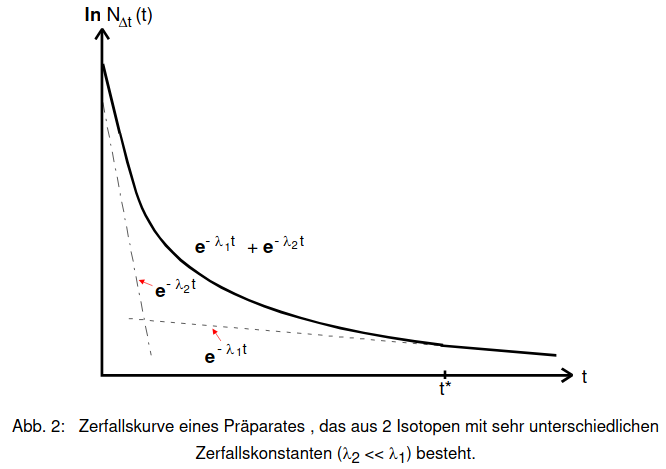
\includegraphics{Kurve.png}
        \label{fig:plot}
    \end{figure}
    $\lambda_l$ kann also aus den Werten $t > t⁺$ mittels Ausgleichsrechnung berechnet werden. 
    Nun wird dieser Wert in GLeichung \ref{eqn:N} eingesetzt und daraus die Werte $N_{\Delta t_l}$
    gewonnen. Substrahiert von den Gesamtzählraten $N_{\Delta t}(t_i)$ liefern sie die Werte für den 
    langsameren Zerfall. Auch hier wird eine Ausgleichsrechnung mit kleinen t (aufgrund von 
    statistischen Schwankungen) zur Bestimmung durchgeführt. 
    
    